%%%%%%%%%%%%%%%%%%%%%%%%%%%%%%%%%%%%%%%%%
% Stylish Article
% LaTeX Template
% Version 2.1 (1/10/15)
%
% This template has been downloaded from:
% http://www.LaTeXTemplates.com
%
% Original author:
% Mathias Legrand (legrand.mathias@gmail.com) 
% With extensive modifications by:
% Vel (vel@latextemplates.com)
%
% License:
% CC BY-NC-SA 3.0 (http://creativecommons.org/licenses/by-nc-sa/3.0/)
% Adaptation: Jens Buysse
%
%%%%%%%%%%%%%%%%%%%%%%%%%%%%%%%%%%%%%%%%%


\documentclass[fleqn,10pt]{voorstel}

\usepackage[english,dutch]{babel}

\usepackage{lipsum}
\usepackage{listings}
\setlength{\columnsep}{0.55cm} % Distance between the two columns of text
\setlength{\fboxrule}{0.75pt} % Width of the border around the abstract

%----------------------------------------------------------------------------------------
%	COLORS
%----------------------------------------------------------------------------------------

\definecolor{color1}{RGB}{0,111,184} % Color of the article title and sections
\definecolor{color2}{RGB}{0,20,20} % Color of the boxes behind the abstract and headings

\lstset{frame=tb,
	language=Command.com,
	aboveskip=3mm,
	belowskip=3mm,
	showstringspaces=false,
	columns=flexible,
	basicstyle={\small\ttfamily},
	numbers=none,
	numberstyle=\tiny\color{gray},
	keywordstyle=\color{gray},
	commentstyle=\color{dkgreen},
	stringstyle=\color{mauve},
	breaklines=true,
	breakatwhitespace=true,
	tabsize=3
}

\usepackage{natbib}
\usepackage{hyperref} % Required for hyperlinks
\hypersetup{hidelinks,colorlinks,breaklinks=true,urlcolor=color1,citecolor=color2,linkcolor=color2,bookmarksopen=false,pdftitle={Title},pdfauthor={Author}}

%----------------------------------------------------------------------------------------
%	ARTICLE INFORMATION
%----------------------------------------------------------------------------------------

\JournalInfo{Hogeschool Gent} % Journal information
\Archive{Onderzoekstechnieken 2015 - 2016} % Additional notes (e.g. copyright, DOI, review/research article)

\PaperTitle{Vergelijkende studie van 3D capaciteiten bij studenten laptops}% Article title

\Authors{Brian Pinsard, Jovi De Croock, Thomas Vansevenant, Dieter Willems} % Authors
%\affiliation{} % Author affiliation

\Keywords{3D Benchmarking --- Graphics --- Physics --- Laptops} % Keywords 
\newcommand{\keywordname}{Keywords} % Defines the keywords heading name


\Abstract{Tekst...

Tekst....
}

%----------------------------------------------------------------------------------------

\begin{document}

\flushbottom % Makes all text pages the same height

\maketitle % Print the title and abstract box

\tableofcontents % Print the contents section

\thispagestyle{empty} % Removes page numbering from the first page

%----------------------------------------------------------------------------------------
%	ARTICLE CONTENTS
%----------------------------------------------------------------------------------------

\section{Introductie} % The \section*{} command stops section numbering
Naar aanleiding van het groeiend aanbod aan games en het een groeiend aantal gamers hebben we een vergelijkende studie van 3D capaciteiten bij studenten laptops gedaan. Hierbij hebben we de laptops van een groepje van 4 studenten (Dieter, Brian, Thomas, Jovi) vergeleken met elkaar om zo te kijken welke laptop er de beste is. 
\subsection{Laptops}
Voor dit onderzoek hebben we de laptops: Acer Aspire E17 (Dieter), MSI GT72 2QE Dominator Pro (Brian), Aspire V3 772G (Thomas), MSI GE60(Jovi) met elkaar vergeleken. Deze laptops werden allemaal met ongeveer dezelfde reden gekocht. Iedereen verkoos een laptop waarmee ze hun school taken zeer effici{\"e}nt kunnen verwezelijken maar toch nog steeds verscheidene multimedia activiteiten kunnen uitvoeren. Hier onder verstaan we spellen, het renderen van 3D modellen, \dots \\
Zie tabel~\ref{gpu-specs} voor de desbetreffende laptops hun GPU specificaties en tabel~\ref{cpu-specs} voor hun CPU specificaties.
\begin{table*}[t]
\centering
\caption{GPU specificaties}
\label{gpu-specs}
\begin{tabular}{lllll}
Laptop naam                & GPU                     & GPU snelheid & GPU geheugen & GPU geheugen snelheid \\
MSI GT72 2QE Dominator Pro & NVIDIA GeForce GTX 980M & 1038 MHz  & 8192 MB    & 1253 MHz         \\
MSI GE60                   & NVIDIA GeForce GT 750M  & 941 MHz   & 2048 MB    & 1003 MHz          \\
Acer Aspire E17            & NVIDIA GeForce 840M     & 1029 MHz  & 2048 MB    & 900 MHz          \\
Acer Aspire V3 772G             & NVIDIA GeForce GT 750M  & 967 MHz   & 4096 MB    & 900 MHz         
\end{tabular}
\end{table*}
\begin{table*}[t]
\centering
\caption{CPU \& Geheugen specificaties}
\label{cpu-specs}
\begin{tabular}{lllll}
Laptop naam				   & CPU                    & CPU kernen     & CPU snelheid	& Geheugen (1600 MHz)  \\
MSI GT72 2QE Dominator Pro & Intel® Core™ i7-4710HQ & 4 (8 virtueel) & 2.50 GHz	& 16384 MB	\\
MSI GE60                   & Intel® Core™ i7-4700MQ & 4 (8 virtueel) & 2.40 GHz	& 8192 MB	\\
Acer Aspire E17            & Intel® Core™ i7-4510U  & 2 (4 virtueel) & 2.00 GHz	& 8192 MB	\\
Acer Aspire V3 772G             & Intel® Core™ i7-4702MQ & 4 (8 virtueel) & 2.20 GHz	& 16384 MB 
\end{tabular}
\end{table*}

%------------------------------------------------

\section{State-of-the-art}
\input{stato}

%------------------------------------------------

\section{Methode van aanpak} \label{sec-moa}
\subsection{Keuze van software}
Na we onze onderzoeksvraag afgebakend hadden, zijn we ons onderzoek gestart met het zoeken van tools die beschikbaar zijn voor het testen van de visuele capaciteiten van een computer. Hierbij sprongen de volgende benchmarking tools uit: FurMark, Unigine en 3DMark.

\subsubsection{Furmark}
Furmark is een zeer intensieve OpenGL benchmark die vooral als stabiliteit en stress test gebruikt word, hierbij word grafische kaart tot zijn uiterste geduwd en kan deze oververhitten. Dit was dus toch geen correcte tool voor onze doeleinden. \citep{furmark}

\subsubsection{3DMark vs Unigine}
Tussen 3DMark en Unigine hebben we gekozen om 3DMark te gebruiken als benchmarking tool. De reden hiertoe is dat 3DMark een zeer bekende tool is en tegenwoordig er ook een gratis versie beschikbaar is via het Steam platform, dit heeft ervoor gezorgd dat ieder groepslid de zelfde versie van 3DMark geinstalleerd staan had.

\subsubsection{3DMark}
3DMark bevat verscheidene benchmarks die elk gericht zijn op een specifieke klasse van hardware dit varieert van smartphones tot gaming computers. Deze benchmarks worden gebruikt door honderden hardware review websites en verscheidene van de hardware fabrikanten.\\\\
Uit de benchmarks die 3DMark beschikbaar stelt hebben we gekozen voor de benchmark “Sky Diver”, deze is geschikt voor gaming laptops tot en met mid-range computers. We hebben voor deze benchmark gekozen omdat dit overeen komt met ons standaard gebruik van de laptops die getest worden. De rendering resolutie staat bijvoorbeeld vast op 1920x1080 bij een benchmark geschikt voor een lagere klasse van apparaten staat deze resolutie vast op 1280x720, de resultaten van die benchmark zouden geen representatieve weergave tegenover daadwerkelijk gebruik van de laptop.

\subsection{3DMark: Sky Diver}
Binnen de benchmark “Sky Diver” zijn er vier testen en een demo die uitgevoerd kunnen worden, wij hebben gekozen om de vier testen uit te voeren omdat de demo niet relevant is tot de eindscore van deze benchmark.

\subsubsection{Grafische testen}
De eerste grafische test maakt gebruik van de forward lighting method met één directioneel licht. Deze traditionele methode gaat elk object apart gaan oproepen en  per lichtbron in de scene deze visualiseren terwijl de belichting berekend word, dit wil zeggen dat deze methode heel duur is qua performantie. Ook word er een depth of field effect toegepast als nabewerking. \citep{3dmark_tech,3dmark_light}

De tweede grafische test focust zich op pixel processing en gebruikt een compute shader-based deferred tile lighting method. Het verschil met de eerste grafische test qua belichting ligt hem in de methode waarbij de objecten nu eerst allemaal gevisualiseerd zullen worden en pas daarna de belichting voor de volledige scene berekend zal worden. Bij deze test word er ook een lens reflectie effect toegepast als nabewerking. \citep{3dmark_tech,3dmark_light}

%De totale grafische score wordt berekend volgens deze formule:
%\[Sgraphics = 219 \times \frac{2}{\frac{1}{Fgt1}+\frac{1}{Fgt5}}\]
%Waar Fgt1 de gemiddelde fps van de eerste grafische test is en Fgt2 de gemiddelde fps van de tweede grafische %test. Zoals beschreven door \cite{3dmark_tech}

\subsubsection{Physics test}
Terwijl de grafische testen vooral de GPU zullen belasten en testen, zal de physics test de CPU testen door 96 standbeelden als objecten neer te slaan met een hamer. Deze hamers hangen vast aan kettingen waardoor de CPU immens veel zal moeten bereken zoals hoe de hamers moeten zwaaien en wanneer de hamers een standbeeld raken hoe de stukken van het standbeeld moeten vliegen. Deze 96 standbeelden worden verdeeld over 4 levels, elk level worder er significant meer standbeelden tegelijk gevisualiseerd en geraakt door één van de hamers, zodat de CPU naarmate de tijd verstrijkt meer zal moeten verwerken. \citep{3dmark_tech}

%De physics score is een gewogen gemiddelde van de twee levels die het best gelukt zijn volgens deze formule:
%\[Sphysics = 56 \times ((1-Wi)N_{i-1}-F_{i-1}+WiNiFi)\]
%Waar W de gewichtsfactor voor een level is, i de index van het laatste level dat gedraaid heeft, N de fps %normalisatie factor voor een level en F de fps van een level. Zoals beschreven door \cite{3dmark_tech}

\subsubsection{Gecombineerde test}
Deze test is een combinatie van de tweede grafische test en het derde level van de phsyics test. Er wordt gebruik gemaakt van een compute shader based deferred tiled lighting method zoals in de tweede grafische test en er worden 48 standbeelden geladen en omgezwaaid door hamers zoals in het derde level van de physics test. De test is ontworpen om een gebalanceerde belasting uit te voeren op zowel de GPU als de CPU. \citep{3dmark_tech}

%De gecombineerde score wordt berekend volgens deze formule:
%\[Scombined = 243 \times Fcombined\]
%Waar:
%\begin{description}
%\item[Fcombined] = gemiddelde fps van de gecombineerde test
%\end{description}
%Zoals beschreven door \cite{3dmark_tech}

\subsection{Workflow}
We hebben gekozen om de bovenstaande vier testen op ieder groepslid zijn laptop 30 keer te laten draaien, het formaat waarin 3DMark standaard de resultaten exporteerd is helaas niet bruikbaar aangezien we de resultaten er niet kunnen uit halen. Hier door hebben we gebruik moeten maken van de command line tools om de resultaten te exporteren naar een bestand van het XML formaat, dit bestand was simpel te converteren met een zelf geschreven Java programma naar een bestand van het XLS formaat zodat we met de resultaten konden beginnen werken.

\subsubsection{Benchmark via command line}
Voor de benchmark via command line te laten draaien hebben we allereerst een custom XML setting bestand aangemaakt waarin de testen worden aangegeven die gedraaid moeten worden en er ook ingesteld word dat de benchmark systeem info moet verzamelen. Hiervoor hebben we onderstaand commando gebruikt:
\begin{lstlisting}
3DMarkCmd.exe --definition=skydiver_custom.3dmdef --export=skydiver_naam.xml --loop=30
\end{lstlisting}
Het commando hebben we opgesteld gebaseerd op de commandos die te vinden zijn in de 3DMark Command Line Guide door \cite{3dmark_cmd}. 
\subsubsection{Converteren van resultaten}
Voor het converteren van het XML bestand naar een XLS bestand hebben we een eigen java programma geschreven dat gebruik maakt van de SAX Parser om het XML bestand om te zetten naar standaard Java objecten en daarna Apache POI om deze objecten weg te schrijven naar een XLS bestand. Het programma kan gebruikt worden via het volgende commando:
\begin{lstlisting}
java -jar 3dmark_results_converter.jar skydiver_naam.xml
\end{lstlisting}
Waar skydiver\_naam.xml het input bestand is, na dit commando uit te voeren zal het programma vragen om een output bestandsnaam te geven. Het XLS bestand met de resultaten wordt nadien gegenereerd.

\subsubsection{Vergelijking van de resultaten}
Bij ieder groepslid zijn resultaten worden de gemiddelden genomen van iedere test zijn 30 testresultaten en deze worden dan verder gebruikt voor...

\section{Resultaten}
In dit deel zullen de resultaten van de testen toegelicht worden, deze zijn onderverdeeld in: de grafische testen, de Physics test en de algemene scores berekend volgens de formules vermeld in sectie 3.

\subsection{Grafische testen}

Deze test legt de nadruk eerder op de grafische processor van de laptop, als we de laptops bekijken dan mogen we vrij zeker zijn dat de MSI GT72 er bovenuit zal steken door zijn nieuwere en sterke grafische kaart. Hier is de bijhorende grafiek: \\
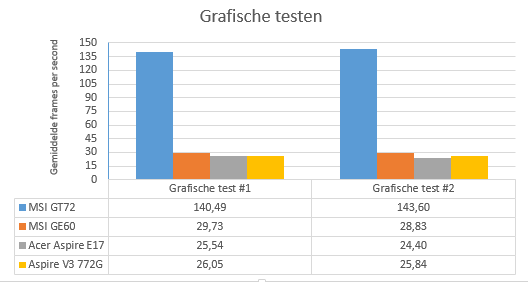
\includegraphics[width=8cm]{grafische}\\
Zoals verwacht steekt de GT72 hier met kop en schouders bovenuit door zijn grafische kaart (GTX980M) deze is voor het moment de nieuwste versie voor de NVIDIA chipset.\\
De GE60 & de Aspire V3 772G dezelfde grafische kaart hebben is er een klein verschil in performantie, de GE60 zijn performantie ligt iets hoger.
Het vreemde is dat de Aspire E17 een nieuwere grafische kaart heeft maar toch een gelijkaardige performantie heeft aan de andere twee, dit komt door dat de GPU's die eindigen met 50 en hoger mid tot high-end zijn maar die eronder worden verondersteld van low-end te zijn.

\subsection{Physics test}

Zoals vermeld in sectie 3 is deze test meer op de Processor gericht, als we naar de tabel kijken zien we dat de GT72 de nieuwste generatie CPU heeft, de GE60 en de Aspire V3 hebben dezelfde generatie CPU en de Aspire E17 heeft een iets zwakkere CPU.\\
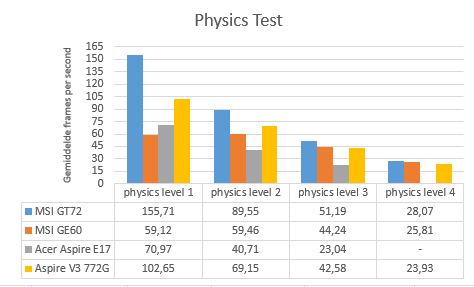
\includegraphics[width=8cm]{physics}\\
Deze test wordt opgedeeld in vier testen zoals vermeld in sectie 3.2.2, we zien dat de GT72 in het eerste level een veel hogere performantie heeft dan de rest, verassend zien we ook dat de GE60 een aanzienlijk lagere score heeft als het om weinig objecten tegelijk draait.
Wanneer we het tweede level bekijken zien we dat de performantie van de Aspire E17 heel hard is afgevallen en dat de GE60 en Aspire V3 min of meer gelijkgekomen zijn maar de Aspire V3 steekt er nog steeds iets boven.
Bij het derde niveau is de GT72 zijn performantie sterk aan het gelijkkomen met die van de GE60 en de Aspire V3 terwijl de Aspire E17 verder afvalt.
Bij het laatste niveau kunnen we concluderen dat deze CPU's weinig onderscheid hebben als het draait om zoveel berekeningen tegelijk. Er is geen resultaat bij level 4 bij de Aspire E17 omdat het aantal frames per seconde dat de laptop haalt onder de minimum threshold valt voor deze test.

\subsection{Scores}


\section{Conclusies}
Tekst...

%----------------------------------------------------------------------------------------
%	REFERENCE LIST
%----------------------------------------------------------------------------------------
\phantomsection
\bibliographystyle{apa}
\bibliography{biblio}

%----------------------------------------------------------------------------------------

\end{document}
